\documentclass[pdflatex,sn-mathphys-num]{sn-jnl}% Math and Physical Sciences Numbered Reference Style

\usepackage{graphicx}%
\usepackage{multirow}%
\usepackage{amsmath,amssymb,amsfonts}%
\usepackage{amsthm}%
\usepackage{mathrsfs}%
\usepackage{xcolor}%
\usepackage{textcomp}%
\usepackage{manyfoot}%
\usepackage{booktabs}%
\usepackage{algorithm}%
\usepackage{algorithmicx}%
\usepackage{algpseudocode}%
\usepackage{listings}%
\usepackage{bm}
\usepackage{xr}

% Cross-references to the main article (compile main.tex first, then this file).
\externaldocument{main}

\renewcommand{\figurename}{Supplementary Figure}
\renewcommand{\tablename}{Supplementary Table}

\raggedbottom

\begin{document}

\title[Supplementary Information]{Supplementary Information for HIP: Hessian Interatomic Potentials without derivatives}

\author[1]{\fnm{Andreas} \sur{Burger}}
\author[1]{\fnm{Luca} \sur{Thiede}}
\author[1]{\fnm{Nikolaj} \sur{R{\o}nne}}
\author[1]{\fnm{Nandita} \sur{Vijaykumar}}
\author[1]{\fnm{Varinia} \sur{Bernales}}
\author[1]{\fnm{Tejs} \sur{Vegge}}
\author[1]{\fnm{Arghya} \sur{Bhowmik}}
\author*[1]{\fnm{Al{\'a}n} \sur{Aspuru-Guzik}}
\affil[1]{Affiliations are given in the main text.}

\maketitle

\section{MLIPs and equivariant neural networks}
Early works on machine learning interatomic potentials used local atomic environment descriptors in combination with linear regression \citep{thompson2015,shapeev2016}, Gaussian processes \citep{bartok2010}, and simple neural networks \citep{behler2007}.
SchNet \citep{schutt2018} was the first work to introduce \textit{rotation-invariant graph neural networks} for predicting molecular properties such as energies and forces. Next-generation invariant architectures include ViSNet \citep{wang2022} and QuinNet \citep{wang2024}.
In parallel, \textit{rotation-equivariant} architectures were developed, such as Cormorant \citep{anderson2019}, DimeNet \citep{gasteiger2020}, GemNet \citep{gasteiger2021}, PaiNN \citep{schutt2021}, NequIP \citep{batzner2022}, SphereNet \citep{liu2022}, MACE \citep{batatia2022} and the Equiformer family \citep{liao2023, liao2023equiformerv2, burger2025dequify}. \\
After several layers of message passing, task-dependent readout heads map the node features to the desired targets while respecting symmetry. For example, energies $E$ are $\mathrm{SO}(3)$-invariant per-graph scalars. The energy readout head therefore uses a global pooling and a reduction operation to output a $l{=}0$ feature. Forces $\mathbf{F}$ are $\mathrm{SO}(3)$ equivariant per-atom vectors ($l=1$), and can be outputted either by a direct force readout head, or as the derivative of the energy $\mathbf{F} = -\nabla_\mathbf{R} E$. Hessians are $\mathrm{SO}(3)$-equivariant per-graph matrices composed of per-atom-pair $3\times3$ equivariant sub-matrices. \\
There is a rich connection between the HIP Hessian prediction in this work and other rotation-equivariant matrices of interest, like Hamiltonian prediction. For example, PhisNet \cite{unke2021se}, QHNet \cite{yu2023efficient}, HELM \cite{Kaniselvan2025helm}, and WANet \cite{li2025enhancing} predicts the Fock matrix, and Graph2Mat \cite{febrer2025graph2mat} targets the density matrix. MōLe \citep{thiede2026mole,burger2026molelambda} predicts coupled cluster amplitudes from Hartree-Fock orbitals.
% 
\section{Traditional methods for calculating Hessians}
\subsection{Analytical Hessians via CPKS}
\label{sec:cpks}
The gold standard for computing nuclear Hessians is to derive them analytically. In Kohn-Sham DFT, this is done with the Coupled Perturbation Kohn-Sham (CPKS) method. This is much more complex and computationally demanding than energy or force calculations. The difficulty arises from the need to calculate the response term of the electron density, which requires understanding how the self-consistent field (SCF) solution to the Kohn-Sham equations changes with changes in nuclear coordinates. To see why this is necessary, write the DFT energy in terms of the density matrix $\mathbf{P}(\mathbf{R}) = (\mathbf{C})^T(\mathbf{R}) \mathbf{S}(\mathbf{R}) \mathbf{C}(\mathbf{R})$ with molecular orbital coefficients $\mathbf{C}$ and overlap matrix $\mathbf{S}$: 
\begin{align}
    E[\mathbf{P}] = \text{Tr}[h\mathbf{P}] + \frac{1}{2} \text{Tr}[\mathbf{J}[\mathbf{P}]] + \rho(\mathbf{P})
\end{align}
To get the force, so the nuclear gradient, we first define the Lagrangian to enforce normalization of the wavefunction:
\begin{align}
\mathcal{L}(C, \epsilon, \mathbf{R}) = E[\mathbf{R}] - \text{Tr}[\epsilon (\mathbf{C}^T\mathbf{S}\mathbf{C} - \mathbf{I})] \label{eq:lagrangian}
\end{align}
We then get the nuclear gradient by differentiating $\mathcal{L}$. The derivative w.r.t. nuclear component $x$ is:
\begin{align}
    \frac{d\mathcal{L}}{dx} &= \frac{\partial\mathcal{L}}{\partial x} + \underbrace{\frac{\partial \mathcal{L}}{\partial \mathbf{C}}}_{=0} \frac{\partial \mathbf{C}}{\partial x} - \text{Tr}\left[\epsilon \mathbf{C}^T \frac{\partial \mathbf{S}}{\partial x} \mathbf{C}\right] + 2 \text{Tr}\left[(\mathbf{S}\mathbf{C}\epsilon)^T\frac{d\mathbf{C}}{dx}\right] \\
    &= \frac{\partial E}{\partial x} - 2 \text{Tr}\left[(\mathbf{S}\mathbf{C}\epsilon)^T\frac{dC}{dx}\right]  -\text{Tr}\left[\epsilon \mathbf{C}^T \frac{\partial \mathbf{S}}{\partial x} \mathbf{C}\right] + 2 \text{Tr}\left[(\mathbf{S}\mathbf{C}\epsilon)^T\frac{d\mathbf{C}}{dx}\right] \\
    &= \frac{\partial E}{\partial x}  -\underbrace{\text{Tr}\left[\epsilon \mathbf{C}^T \frac{\partial \mathbf{S}}{\partial x} \mathbf{C}\right]}_\text{"Pulay terms"} \label{eq:analytic_grad}
\end{align}
Due to the stationarity $\frac{\partial \mathcal{L}}{\partial C} = 0$ we did not need to calculate the density response $\frac{\partial C}{\partial x}$, which is why calculating forces is cheap, on the same order as the cost of energies. However, once we want Hessians, we need to differentiate \eqref{eq:lagrangian} twice:
\begin{align}
    \frac{d^2 \mathcal{L}}{dx dy} &= \frac{\partial^2 \mathcal{L}}{\partial x \partial y} + \frac{\partial^2 \mathcal{L}}{\partial \mathbf{C} \partial x} \frac{d \mathbf{C}}{d y} + \frac{\partial^2 \mathcal{L}}{\partial \epsilon \partial x}\frac{d \epsilon}{dy} \\
    &=  \frac{\partial^2 \mathcal L}{\partial y\,\partial x}
-\begin{bmatrix}
\displaystyle \frac{\partial^2 \mathcal L}{\partial \mathbf{C}\,\partial x} &
\displaystyle \frac{\partial^2 \mathcal L}{\partial \varepsilon\,\partial x}
\end{bmatrix}
\begin{bmatrix}
\displaystyle \frac{\partial^2 \mathcal L}{\partial \mathbf{C}^2} & \displaystyle \frac{\partial^2 \mathcal L}{\partial \mathbf{C}\,\partial \varepsilon} 
\displaystyle \frac{\partial^2 \mathcal L}{\partial \varepsilon\,\partial \mathbf{C}} & \displaystyle \frac{\partial^2 \mathcal L}{\partial \varepsilon^2}
\end{bmatrix}^{-1}
\begin{bmatrix}
\displaystyle \frac{\partial^2 \mathcal L}{\partial \mathbf{C}\,\partial y} 
\displaystyle \frac{\partial^2 \mathcal L}{\partial \varepsilon\,\partial y}
\end{bmatrix}.
\end{align}
Solving the linear system of equations scales formally as $O(N^5)$ in computation and $O(N^4)$ in memory. Similar to energy calculations, density fitting, sparsification (integral screening), and other optimizations can reduce the cost for CPKS. Still, the scaling remains worse in both computation and memory compared to energy calculations. 

\subsection{Hessians via finite differences}
\label{sec:finite_difference}
A major downside of the CPKS approach to Hessians is its highly complex implementation and need for exchange-functional-specific derivations. Therefore, many new methods do not support Hessians, and most codes resort to finite-difference calculations in such cases. Using central differences of the forces along the $3N$ Cartesian directions, the Hessian elements are constructed from
\begin{align}
    \mathbf{H}_{ij} \approx \frac{\mathbf{F}_i(\mathbf{R} + h \mathbf{e}_j) - \mathbf{F}_i(\mathbf{R} - h \mathbf{e}_j)}{2h}
\end{align}
This requires $2\times 3N$ displaced \emph{gradient} calculations. Each gradient calculation scales similarly to the energy calculation with $O(N^4)$, leading to a $O(N^5)$, the same as naive CPKS, although typically with more numerical noise and a much larger prefactor because we have to repeatedly converge an SCF, as opposed to solving a large linear system in analytical Hessians.
% 
\subsection{Hessians from MLIPs}
MLIPs have gained widespread popularity for their ability to accurately approximate molecular energies and forces. The forces can either be directly predicted \citep{gasteiger2021, liao2023equiformerv2}, or calculated as the derivative of the MLIP energy using automatic differentiation. %, with a cost of about 2-3 times that of an energy forward pass. 
Previous work has shown that the Hessian can be calculated using AD to some success \citep{yang2024, yuan2024, gonnheimer2025, rodriguez2025, williams2025, cui2025horm}. 
Although AD Hessians are much cheaper to calculate compared to DFT, they come with two major downsides.
%A natural question then is to ask if we can also calculate the Hessian cheaply by simply differentiating the energy twice. In principle, the answer is yes, but with some nuances:
First, accurately modeling the energy and forces does not guarantee low Hessians errors \citep{yuan2024}, but requires dedicated training \citep{zhao2025, cui2025horm}. 
Similar to how adding force labels dramatically improves autograd forces over energy-only training \cite{christensen2020forces}, we need Hessian labels in practice for accurate autograd Hessians.
Second, autograd Hessians are expensive.
Since the Hessian is the derivative of the force with respect to the $3N$ atom coordinates, the cost of one autograd Hessian is $3N$ times the cost of a regular MLIP forward pass.
Assuming the force calculation with an MLIP is usually $O(N)$ to $O(N^2)$, the total cost of the Hessian calculation is $O(N^2)$ to $O(N^3)$ in time and memory. 
%Automatic differentiation calculates the Hessian via Hessian-Vector-Products (HVPs). 
%Given a probing vector $\mathbf{v}_i = \mathbf{e}_i, i=0,...,3N-1$, AD allows us to calculate the $i$-th column of the Hessian with $\mathbf{H}\mathbf{v}_i$. 
Formally, to calculate the full $3N\times 3N$ Hessian, one needs $3N$ Hessian vector products (HVPs) with the unit vectors $\mathbf{v} = \mathbf{e}_i, i=0,...,3N-1$, each yielding one column of the Hessian. 
While the HVPs can theoretically be parallelized, the $O(N^2)$-$O(N^3)$ memory footprint requires even medium-sized systems to be computed sequentially.
Alternatively, we can obtain Hessians using finite differences \citep{gonnheimer2025, fu2025, wander2025accessing}, which requires less memory but $6N$ forward passes.
\cite{rodriguez2025} in particular showed that including the Hessian in the loss leads to better extrapolation of energy and force predictions, less data for a given accuracy, and improved stability in MD. This comes at the cost of approximately 25$\times$ longer training times, which makes AD Hessians prohibitive to train.

\section{Hessians in Molecular Optimization}

\subsection{Geometry optimization \label{sec:optimizerliterature}}
Geometry optimization locates minima $\arg\!\min_\mathbf{R} E(\mathbf{R})$ of the potential energy surface starting from non-equilibrium molecular geometries. It underpins most workflows from global searches\cite{christiansen2022,ronne2022} to high-throughput screening\cite{westermayr2023,ronne2024}. 
The efficiency of geometry optimization depends on four key factors: (i) the choice of coordinate system, (ii) the quality of the Hessian approximation, (iii) the update strategy, and (iv) the step size control. 
Cartesian coordinates are straightforward but strongly coupled, limiting step size and slowing convergence for flexible systems. In contrast, internal coordinates are better aligned with chemically meaningful motions, separate stiff and soft modes, and allow constraints to be imposed naturally. These properties often lead to substantially fewer iterations. 
Some of the most widely used optimizers are the first-order FIRE \citep{bitzek2006} optimizer and the second-order rational function optimization (RFO) optimizer.
% Most nonlinear optimization algorithms are based on a local quadratic expansion around an initial geometry 
% $\mathbf{R}_0$, 
% \begin{equation}
% E(\mathbf{R}) \approx 
% E(\mathbf{R}_0) + \mathbf{F}_0^\top \Delta\mathbf{R} 
% + \tfrac12 \Delta\mathbf{R}^\top H_0 \Delta\mathbf{R},
% \end{equation}
% where $\mathbf{F}_0 = F(\mathbf{R}_0)$ is the force and $H_0$ the Hessian at $\mathbf{R}_0$. The displacement $\Delta \mathbf{R}$ is obtained by using the exact Hessian or by iteratively improving an approximation.

\subsubsection{RFO \label{sec:rfo_background}}
Rational function optimization (RFO) \citep{simons1983,banerjee1985} is a commonly used second-order optimization technique in molecular geometry optimization. RFO starts with a [2/2]-Pad\'e-expansion of the energy:
\begin{align}
    E(\mathbf{R_t} + \Delta \mathbf{x}) - E(\mathbf{R_t}) \approx \frac{\mathbf{g}^\top \Delta \mathbf{x} + \frac{1}{2} \Delta \mathbf{x}^\top \mathbf{H} \Delta \mathbf{x}}{1 + |\Delta\mathbf{x}|^2 }
\end{align}
The extrema $\Delta x'$ of this surrogate are given by the solution of the generalized eigenvalue problem:
\begin{align}
\begin{bmatrix}
    \mathbf{H} & \mathbf{g} \\
    \mathbf{g}^\top & 0
\end{bmatrix}
\begin{bmatrix}
    \Delta \mathbf{x}' \\
    1
\end{bmatrix}
=
\lambda
\begin{bmatrix}
    I & 0 \\
    0 & 1
\end{bmatrix}
\begin{bmatrix}
    \Delta \mathbf{x}' \\
    1
\end{bmatrix}. \label{eq:augmented_eig}
\end{align}
An attractive property of RFO is that it can be used both for minimizing $E(\mathbf{R})$ as well as for finding saddle points (important for transition state search, we use the restricted step RFO (RS-RFO) for minimization \ref{eq:augmented_eig}, we get an update pointing to the minimum; if we select the second eigenvector, we get a transition state update. In contrast to Newton-Raphson optimization, RFO is also robust to indefinite Hessians. For detailed derivation, see \citep{simons1983, banerjee1985}. In this paper, for minimization, we are using restricted step RFO (RS-RFO), which adds a trust region to prevent unphysically large steps. For the transition point search, we are using restricted step partitioned RFO (RS-P-RFO), a slight modification that treats the subspaces with negative and positive Hessian eigenvalues separately.
% Since computing the exact Hessian is prohibitively expensive for all but the smallest systems, quasi-Newton methods construct an approximate Hessian that is updated using gradient differences.
% Several widely used algorithms embody different choices of these ingredients. The BFGS method provides a robust quasi-Newton update scheme and is routinely applied in both Cartesian and internal coordinates.

\subsubsection{BFGS}
\label{sec:bfgs}
To apply RFO in practice, we need a Hessian at each step. As computing full Hessians is usually too expensive, a common practice is to maintain an approximate Hessian using the BFGS quasi-Newton scheme. BFGS updates approximate Hessians $\mathbf{B}_k$ of the true Hessian $\mathbf{H}(\mathbf{R}_k)$ using the update equation
\begin{align}
    \mathbf{B}_{k+1} = \mathbf{B}_k 
    - \frac{\mathbf{B}_k \mathbf{s}_k \mathbf{s}_k^\top \mathbf{B}_k}{\mathbf{s}_k^\top \mathbf{B}_k \mathbf{s}_k}
    + \frac{\mathbf{y}_k \mathbf{y}_k^\top}{\mathbf{y}_k^\top \mathbf{s}_k},
    \qquad \mathbf{y}_k^\top \mathbf{s}_k > 0,
\end{align}
where the curvature condition $\mathbf{y}_k^\top \mathbf{s}_k>0$ (typically ensured by a Wolfe line search) guarantees that $\mathbf{B}_{k+1}$ remains positive-definite, which is desirable for minimization. In the RFO framework, $\mathbf{B}_k$ simply replaces the exact Hessian $\mathbf{H}$ in the augmented eigenvalue problem in \eqref{eq:augmented_eig}.

\subsection{Transition State Search \label{sec:tssearchliterature}}
%Why are they useful, details
%Transition state search methods, growing string method, gentlest ascend dynamics, notch elastic band
Transition states are first-order saddle points on the PES. They represent the maximum barrier along the minimum energy path (MEP) between two minima. Identifying transition states is crucial for understanding reaction mechanisms and mapping reaction networks. A first-order saddle point is characterized by having exactly one negative eigenvalue of the Hessian. Over the years, various computational methods have been developed to describe MEPs and locate transition states. \\
Computational methods for transition state search can broadly be categorized as \textit{single-ended} and \textit{double-ended}. In double-ended methods, we know the product and reactant states (the two minima on the energy surface) and seek an interpolation along the MEP that passes through the TS. In contrast, in single-ended methods, we only know a starting point and climb the energy surface to find a nearby transition state. Often, double-ended methods are used to give good initial guesses, which are then refined by single-ended methods. In this study, we use the Growing String method to find the initial states, which we then refine using RS-P-RFO (see above).\\
Different double-ended methods are distinguished by how they grow the interpolations between product and reactant states. The most common approaches are the nudge elastic band method \citep{henkelman1999, henkelman2000} and the growing string method (GSM) \citep{peters2004,zimmerman2015}. 
% Here, we only review the growing string method as we use it in our experiments for the initial guesses of the transition states.


The nudged elastic band method aims to find the minimum energy path between given initial and final configurations. A set of images connecting these states is linked by classical spring forces, forming an elastic band. Each image experiences a total force comprising the spring force along the local tangent and the true force perpendicular to it. The images are simultaneously optimized to trace the MEP. To converge to the transition state, a climbing image is introduced, for which the force along the band is inverted, leaving only the perpendicular component of the true force. This drives the climbing image up the potential energy surface along the band while descending perpendicularly, reaching the transition state along the MEP.

The growing string method (GSM) locates transition states by incrementally constructing a discrete path of structures on the potential energy surface. Starting from the reactant and product endpoints, two path fragments are iteratively grown together. At each iteration, a new node on the string is added along the local tangent direction and relaxed orthogonally to the path according to the force
\begin{equation}
\mathbf{F}_{\bot} = \mathbf{F} - (\hat{\mathbf{t}}^{\top} \mathbf{F}) \hat{\mathbf{t}},
\end{equation}
where $\mathbf{F} = -\nabla E$ is the force and $\hat{\mathbf{t}}$ is the local tangent unit vector. Convergence is typically accelerated by approximate Hessians, constructed in delocalized internal coordinates and updated by quasi-Newton schemes, which enable eigenvector-guided optimization while avoiding full second-derivative evaluations \citep{zimmerman2015}. Once the two fragments merge, the full string is reparameterized to maintain uniform node distance, and the highest-energy node serves as a transition state estimate, which can be further refined using Hessian-based eigenvectors \citep{peters2004}.

\subsection{Frequency analysis for extrema classification}
The final step in a transition state search or minima optimization is to confirm convergence via frequency analysis. A transition state is identified by the Hessian having exactly one negative eigenvalue (or equivalently, one imaginary frequency of the mass-weighted Hessian), whereas a minimum contains no imaginary frequencies. 
To carry out frequency analysis, one must first remove the five or six redundant degrees of freedom, corresponding to the invariance of the energy under rotation and translation. This is done by mass-weighing the Hessian and performing an Eckart projection \citep{louck1976}. Then, the projected matrix is decomposed into its eigenvalues, with all positive eigenvalues indicating a minimum and exactly $N$ negative eigenvalues indicating the presence of an order-$N$ transition state. 

\subsection{Zero-point energy}
Zero-point corrections account for the quantum mechanical vibrational energy that molecules have at absolute zero temperature. To calculate the ZPE, one relaxes a geometry to an extrema, computes the Hessian, and sums the frequencies
% \begin{align}
$ZPE = \frac{\hbar}{2} \sum_i \sqrt{\tilde{\lambda}_i}$.
% \end{align}
Here, $\tilde{\lambda}_i$ are eigenvalues of the mass-weighted Hessian $\mathbf{\tilde{H}}_{AB} = \mathbf{H}_{AB}/m_Am_B$, and $\hbar$ is Planck's reduced constant.
% The ZPE is added to the total energy in many calculations that involve thermodynamic estimates.
One is usually interested in the relative ZPE between reactant and product states: $\Delta ZPE = ZPE(\mathbf{R}_R) - ZPE(\mathbf{R}_P)$. The relative ZPE is relevant for reaction thermochemistry, as $\Delta ZPE$ enters as a correction to the reaction free energy $\Delta G$ and therefore the equilibrium constant, which relates forward and backward rates via detailed balance.
% For reaction rates (Eyring/TST), the relevant quantity is the ZPE correction to the barrier: ΔZPE‡ = ZPE(TS) − ZPE(reactant). This shifts ΔG‡ and thus k ∝ exp(−ΔG‡/kBT).

\section{Hessian properties}
\label{sec:hessian_properties}
The Hessian is a symmetric matrix $\mathbf{H}=\mathbf{H}^\top$ where each sub-block transforms under rotation as a Cartesian tensor
\begin{align}
    \mathbf{H}_{I,J} \xrightarrow[]{\mathbf{Q}} \mathbf{Q} \mathbf{H}_{I,J} \mathbf{Q}^\top 
    % \label{eq:hessian_symmetry}
\end{align}
or equivalently
\begin{align}
    \mathbf{H} \xrightarrow[]{\mathbf{Q}} (\mathbf{I}_{N} \otimes \mathbf{Q})\mathbf{H} (\mathbf{I}_{N} \otimes \mathbf{Q})^\top 
\end{align}
The symmetry follows directly from Schwarz's theorem, which states that for every scalar function $E(\mathbf{R})$ that has continuous partial second derivatives in the neighborhood of a point $\mathbf{R_0}$, the partial second derivatives commute
\begin{align}
    \left(\frac{\partial^2 E}{\partial \mathbf{R}_i \partial \mathbf{R}_j}\right)_{\mathbf{R}=\mathbf{R_0}} = \left(\frac{\partial^2 E}{\partial \mathbf{R}_j \partial \mathbf{R}_i}\right)_{\mathbf{R}=\mathbf{R_0}}
\end{align}
The transformation law under rotation follows straightforwardly from the chain rule: 
First, write the rotated coordinates as
\begin{align}
    \mathbf{R}' &= (\mathbf{I}_{N} \otimes \mathbf{Q}) \mathbf{R} 
    \frac{\partial \mathbf{R}'}{\partial \mathbf{R}} &= (\mathbf{I}_{N} \otimes \mathbf{Q})
\end{align}
Then, define the energy in the rotated frame
\begin{align}
    E'(\mathbf{R}') = E((\mathbf{I}_{N} \otimes \mathbf{Q})^\top \mathbf{R}') = E(\mathbf{R})
\end{align}
Then the first order derivative is
\begin{align}
    \nabla_\mathbf{R'}E'(\mathbf{R'}) &= (\mathbf{I}_{N} \otimes \mathbf{Q}) \nabla_\mathbf{R} E'(\mathbf{R}') \\
    &= (\mathbf{I}_{N} \otimes \mathbf{Q}) \nabla_\mathbf{R} E((\mathbf{I}_{N} \otimes \mathbf{Q})^{-1} (\mathbf{I}_{N} \otimes \mathbf{Q}) \mathbf{R}') \\
    &= (\mathbf{I}_{N} \otimes \mathbf{Q}) \nabla_\mathbf{R} E(\mathbf{R})
\end{align}
showing the equivariance of the forces. The second-order derivative is
\begin{align}
    \mathbf{H}' = \nabla^2_\mathbf{R'} E'(\mathbf{R'}) &= \nabla_\mathbf{R'} ((\mathbf{I}_{N} \otimes \mathbf{Q})\nabla_\mathbf{R}E(\mathbf{R})) \\
    &=(\mathbf{I}_{N} \otimes \mathbf{Q})\nabla_\mathbf{R'}\nabla_\mathbf{R}E(\mathbf{R}) \\
    &=(\mathbf{I}_{N} \otimes \mathbf{Q})\nabla_\mathbf{R}\nabla_\mathbf{R}E(\mathbf{R}) (\mathbf{I}_{N} \otimes \mathbf{Q})^\top \\
    &=(\mathbf{I}_{N} \otimes \mathbf{Q})\mathbf{H} (\mathbf{I}_{N} \otimes \mathbf{Q})^\top
\end{align}
which shows the Hessian's equivariance. 

\subsection{Non-integrability of Hessians\label{sec:conservative}}
% \section{Our Approach: Direct prediction of Hessians}
% We propose to directly predict Hessians with an equivariant neural network, instead of relying on automatic differentiation of an MLIP model. Similar ideas have been proposed for direct force predictions before \citep{gasteiger2021, liao2023equiformerv2}. While direct force predictions achieved low errors on benchmarks, they fell out of popularity for two reasons: 1) The main downstream application for MLIP forces is in MD simulations. Directly predicting forces means that the vector field is not guaranteed to be conservative, though, which causes MD-simulations to dissipate energy over time, leading to wrong observables. 2) The speed-up of direct force-prediction is rather modest. Backpropagation takes "only" about 2x-3x the time of a forward pass. 
% We argue that the situation is different for Hessians: 1) None of the most important use cases of Hessians rely on lengthy simulations where errors could accumulate. Instead, we usually only need Hessians at single points or for short optimizations. We will demonstrate that our directly predicted Hessians not only yield low errors on benchmarks but also achieve excellent performance on the most popular downstream applications. 2) Second-order automatic differentiation is much more expensive than first-order, as we will discuss below. Therefore, the savings for direct Hessian predictions are much larger.
Instead of relying on automatic differentiation, we propose to directly predict Hessians with an equivariant neural network. Similarly, direct force prediction has been proposed before \citep{gasteiger2021, liao2023equiformerv2}. 
While direct force prediction introduces non-integrable errors (non-conservative fields), these errors only cause unbounded blowups when integrated over time, as in Molecular Dynamics (MD). In contrast, for geometry optimization and standard Hessian applications (ZPE, transition state search, preconditioning), these errors remain bounded and merely limit convergence precision rather than accumulating. Therefore, direct Hessian predictions are safe for mainstream computational chemistry tasks, analogous to widely used but non-integrable methods like BFGS.

Since direct Hessian predictions are not formulated as derivatives, they are not guaranteed to be integrable. It is important to understand when a non-integrability error can lead to catastrophically wrong downstream predictions similar to direct force predictions in MD simulations. 
Let's first review the more familiar case: Why do direct force predictions fail in MD simulations but succeed in geometry optimization? Suppose we directly predict forces with error $e(x)=F_\text{pred}(x) - F(x)$. We can decompose the error in a conservative and a non-conservative field using the Helmholtz decomposition: $e(x) = \nabla \phi(x) + S(x)$. $\phi\in \mathbb{R}$ is a scalar potential, and S is a vector field $S(x) \in \mathbb{R}^{3N}$ that is divergence-free $\nabla \cdot S(x) = 0$ but not curl-free $\exists x \text{ s.t. } \nabla \times S(x) \neq 0$.
Now consider how the energy of the system changes over time in an MD simulation:
$$
\begin{aligned}
\Delta E' &= \int_0^T F_\text{pred}(x(t)) v(t) dt = \int_0^T (F(x(t) + e(x(t))) v(t) dt \\
&= \int_0^T (F(x) + \nabla \phi(x) + S(x))v(t) dt \\ 
&= E(T) - E(0) + \underbrace{\phi(T) - \phi(0)}_{\text{ error bounded with time}} + \underbrace{\int_0^T S(x) v(t) dt}_{\text{error unbounded with time}}
\end{aligned}
$$
Since MD simulations use large $T$, non-conservative forces lead to the blowups in error. 

In geometry optimization we define $E' = E + \phi$, then follow the gradient descent ODE:
\begin{align}
\frac{dE'(x(t))}{dt} &= \nabla E'(x(t)) \cdot \frac{d x(t)}{dt} \\
&= -\nabla E'(x(t)) \cdot (\nabla E(x) + e(x)) \\
&= -\nabla E'(x(t)) \cdot (\nabla E(x) + \nabla\phi(x) + S(x)) \\
&= -\nabla E'(x(t)) \cdot (\nabla E'(x)  + S(x)) \\
&= -|\nabla E'(x(t))|^2 + \nabla E'(x) \cdot S(x)
\end{align}
Using the general inequality $2ab \leq a^2 + b^2$:
\begin{align}
\frac{dE'(x(t))}{dt} &= -|\nabla E'(x(t))|^2 + \nabla E'(x) \cdot S(x) \\
&\leq -|\nabla E'(x(t))|^2 + \frac{1}{2}|\nabla E'(x(t))|^2 + \frac{1}{2}|S(x)|^2 \\
&=-\frac{1}{2}|\nabla E'(x(t))|^2 + \frac{1}{2}|S(x)|^2
\end{align}
Therefore, as long as $|\nabla E'(x(t))|^2 > |S(x)|^2$, the direct predicted force minimizes the energy plus some error potential similar to AD forces. Once we are close to convergence, we have $|\nabla E'(x(t))|^2 \leq |S(x)|^2$ and stop converging or enter a limit cycle. This means, we will converge to an extrema on an energy surface $E'$ within a distance of $O(|S|)$. In practice, we are interested in how close we converge to the extrema of the DFT energy $E$. For this, it does not matter if the error stems from the error potential $\phi$ shifting the extrema, or $S$ inducing a small limit cycle. 
As there is no time-dependent error blow-up, it is therefore safe to use direct forces for geometry optimization. 

Now we can do the same for the directly predicted Hessian $H_\text{pred}(x) = H(x) + e(x)$:
Denote the error again as $e(x) = \nabla^2\phi(x) + S(x)$. 
As before, we would get errors scaling with integration length if we tried to calculate quantities of the form
\begin{align}
Q(T) = \int_0^T f(x(t),  H_\text{pred}(x(t))) dx(t)
\end{align}
leading to large errors for large $T$. 

The key advantage is that one of the mainstream tasks integrates over a function of the Hessian for large $T$.

ZPE and geometry classification are single-point calculations; therefore, the errors $\nabla^2\phi(x)$ and $S(x)$ both behave the same, one error is not "worse" than the other. 
Mode following during the transition state search is equivalent to the geometry-optimization analysis with direct forces above. Energy minimization with the Hessian preconditioner is also unproblematic, as the preconditioner cannot change the minimum; it only changes the convergence speed. 

In fact, it is common practice to use BFGS updates for transition state search and energy minimization, and BFGS updates do not have any notion of integrability either.

\section{Batched AD Hessian performance}
\label{sec:batched_ad_explanation}
To test the performance of batched Hessians, we measure the inference time per processed sample for increasingly larger batch sizes and plot the results in \ref{fig:batch_timing}.
\begin{figure}
    \centering
    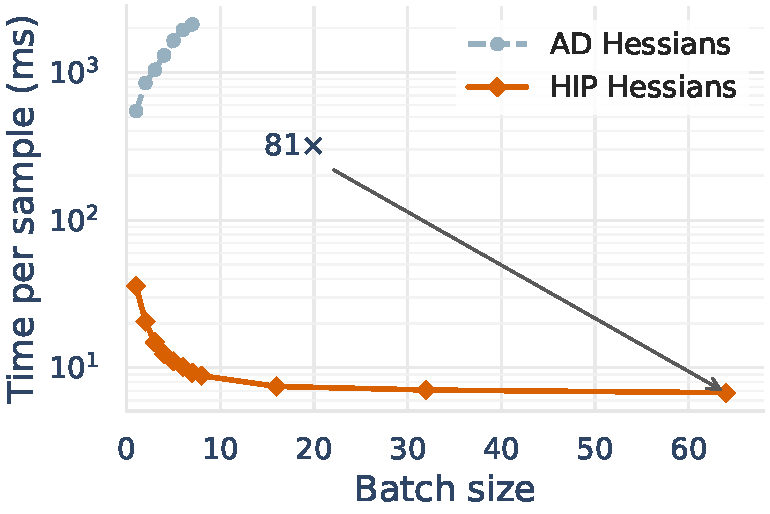
\includegraphics[width=0.5\linewidth]{plots/time_batching.png}
    \caption{\textbf{Compute scaling of HIP compared to AD.} We are measuring the time per sample it takes for increasingly larger batch size. While HIP becomes faster per sample as it efficiently parallelizes, AD becomes slower.}
    \label{fig:batch_timing}
\end{figure}
We observe rapid degradation in the AD Hessian speed with increasing batch size. To explain this, we have to understand exactly how AD treats Hessians. From the point of view of the AD engine, there is no difference between a batch of two molecules of system size $N_A$ and $N_B$, and a larger system of size $N_A + N_B$. In both cases, the MLIP function takes in an array of dimension $3N_A + 3N_B$, and returns either a single scalar $E_A + E_B$ or even worse, an array $[E_A, E_B]$, so mathematically the energy function looks like $E(\mathbf{R}): \mathbb{R}^{3N_A + 3N_B} \rightarrow \mathbb{R}$ or $E(\mathbf{R}): \mathbb{R}^{3N_A + 3N_B} \rightarrow \mathbb{R}^2$. Consequently, a Hessian of this function is a block diagonal matrix of dimension $3(N_A + N_B) \times 3(N_A + N_B)$, or even $2\times 3(N_A + N_B) \times 3(N_A + N_B)$. Therefore, the memory costs grow quadratically with the batch size. Since we have to implement the Hessian calculation using sequential Hessian-Vector products to avoid running out of memory, we cannot even take advantage of parallelization in batched Hessian processing.




\section{Additional results}
\begin{figure}
    \centering
    \includegraphics[width=0.99\linewidth]{plots/hessian_heatmap_idx12345.png}
    \caption{\textbf{HIP compared to ground-truth DFT Hessian.} The horizontal and vertical axis index the $(3N_{Atoms})^2$ entries of the Hessian. We depict the absolute values of test sample C5H6O in eV/\AA$^2$.}
    \label{fig:hessian_heatmap}
\end{figure}

\subsection{Loss function\label{sec:lossablation}}
We are trying to design a loss function that emphasizes the lowest lying eigenvalues/eigenvectors.
To design such a loss function, one could naively compute a loss directly as $L= \sum_i^k |\mathbf{v}_i^\text{predict} - \mathbf{v}_1^\text{true}|$. This requires computing the eigenvalues and eigenvectors of the true and predicted Hessian via an eigenspectrum decomposition. Unfortunately, backpropagation through such an eigenspectrum decomposition is numerically unstable \citep{aaComputationEigenvalueEigenvector2007}.
First, gradients computed using the eigenvectors tensor will only be finite when $\mathbf{H}$ has distinct eigenvalues. Furthermore, if the distance between any two eigenvalues is close to zero, the gradient will be highly sensitive, as it depends on the eigenvalues $\lambda_i $ through the computation of
$
\min_{i \neq j} \frac{1}{\lambda_i - \lambda_j}
$.
Instead, we propose the following subspace loss.

In the following section, we compare the eigenspace loss that we introduced in \eqref{eq:eigenloss} to the standard choice of mean square error (MSE) and mean absolute error (MAE). 

In particular, we emphasize the subspace $k=8$. This is because transition state search, ZPE, and frequency analysis for extrema classification all depend on the two lowest-lying eigenvectors and eigenvalues. We choose $k=8$ instead of $k=2$ to account for the usual $6$ redundant degrees of freedom, which we do not remove during training for numerical stability.

We combine the subspace loss with MAE, so the total loss becomes
\begin{align}
    \mathcal{L}_\text{MAE+Sub} 
    &= \mathcal{L}_\text{MAE} + \mathcal{L}_\text{sub}^{(k=8)} \\
    &=
    \sum_{i,j} |\mathbf{H}_{i,j} - \mathbf{H}^\text{pred}_{i,j}|
     + \sum_{i,j} \left|\mathbf{V}_{[:,:k]}^\top \mathbf{H}^\text{pred}\mathbf{V}_{[:,:8]} - \mathbf{\Lambda}_{[:,:8]}\right|_{i,j} 
     % + \gamma \sum_{i,j} \left|\mathbf{V}_{[:,k:]}^\top \mathbf{H}^\text{pred}\mathbf{V}_{[:,k:]} - \mathbf{\Lambda}_{[:,k:]}\right|_{i,j}
\end{align}
For simplicity, we weight both the MAE and subspace loss equally. Future work could benefit from carefully tuning the relative weights between the loss terms.

On downstream tasks, subspace loss improves over MAE and MSE in (i) transition state search, as shown in Table \ref{tab:loss_tssearch}, and (ii) transition state identification frequency analysis, as shown in Table \ref{tab:loss_freqanalysis}. We observe equal performance between MAE and the subspace loss for (i) geometry relaxation Table \ref{fig:loss_relax} and (ii) computing the zero-point energy Table \ref{tab:loss_zpe}.

Table \ref{tab:loss_acc} shows that the subspace loss improves the first eigenvector $\bm{v}_1$ cosine similarity, and the second eigenvalue $\lambda_2$ MAE. This is consistent with the better performance of the subspace loss on transition state-related tasks, since the transition state is characterized via the two smallest eigenvalues $\lambda_1, \lambda_2$, and is found by following the first eigenvector $\bm{v}_1$.

MSE generally underperforms compared to MAE and MAE with subspace loss.
MSE has the theoretical advantage of being rotation-invariant, whereas MAE is not.
In practice, however, we find that the MSE leads to a high variance (spikes) in the training loss and gradient norm across batches. We speculate that MAE outperforms MSE due to training stability.

Hessian prediction with any loss function tested significantly outperforms prior AD Hessians.

% Accuracy
\begin{table}
\centering
\resizebox{0.99\textwidth}{!}{
\centering
% \begin{tabular}{llccccc}
% \hline
% \multirow{2}{*}{Loss} & \multirow{2}{*}{Model} & Hessian $\downarrow$  & Eigenvalues $\downarrow$ & CosSim $\bm{v}_1$ $\uparrow$ & $\lambda_1$ $\downarrow$ & Time $\downarrow$ 
%  & & eV/\AA$^2$ & eV/\AA$^2$ & unitless & eV/\AA$^2$ & ms 
% \hline
% MSE & EquiformerV2 & 0.033 & 0.072 & 0.728 & 0.168 & 38.7 
% MAE & EquiformerV2 & \textbf{ 0.026 } & \textbf{ 0.057 } & 0.825 & \textbf{ 0.127 } & 38.6 
% MAE+Sub & EquiformerV2 & 0.030 & 0.063 & \textbf{ 0.870 } & 0.130 & 38.5 
\begin{tabular}{lccccccccc}
\hline
\multirow{2}{*}{Loss}  & Hessian $\downarrow$  & Eigenvalues $\downarrow$ & CosSim $\bm{v}_1$ $\uparrow$ & $\lambda_1$ $\downarrow$ & $\lambda_2$ $\downarrow$ & $\lambda_1^{E}$ $\downarrow$ & $\lambda_2^{E}$ $\downarrow$ & CosSim $\bm{v}_1^{E}$ $\uparrow$ & CosSim $\bm{v}_2^{E}$ $\uparrow$ \\
 & eV/\AA$^2$ & eV/\AA$^2$ & unitless & eV/\AA$^2$ & eV/\AA$^2$ & eV/\AA$^2$ & eV/\AA$^2$ & unitless & unitless \\
\hline
MSE  & 0.033 & 0.072 & 0.728 & 0.168 & 0.088 & 0.037 & 0.013 & 0.959 & 0.928\\
MAE  & \textbf{ 0.026 } & \textbf{ 0.057 } & 0.825 & \textbf{ 0.127 } & 0.052 & \textbf{ 0.031 } & 0.012 & 0.976 & 0.952 \\
MAE+Sub  & 0.030 & 0.063 & \textbf{ 0.870 } & 0.130 & \textbf{ 0.030 } & 0.031 & \textbf{ 0.010 } & \textbf{ 0.980 } & \textbf{ 0.957 } \\
\hline
\end{tabular}
}
\caption{Accuracy of HIP-EquiformerV2 using different loss functions. Superscript $E$ denotes after removing redundant degrees of freedom using Eckart-projection on the mass-weighted matrix.}
\label{tab:loss_acc}
\end{table}

% Second order optimization
\begin{figure}
    \centering
    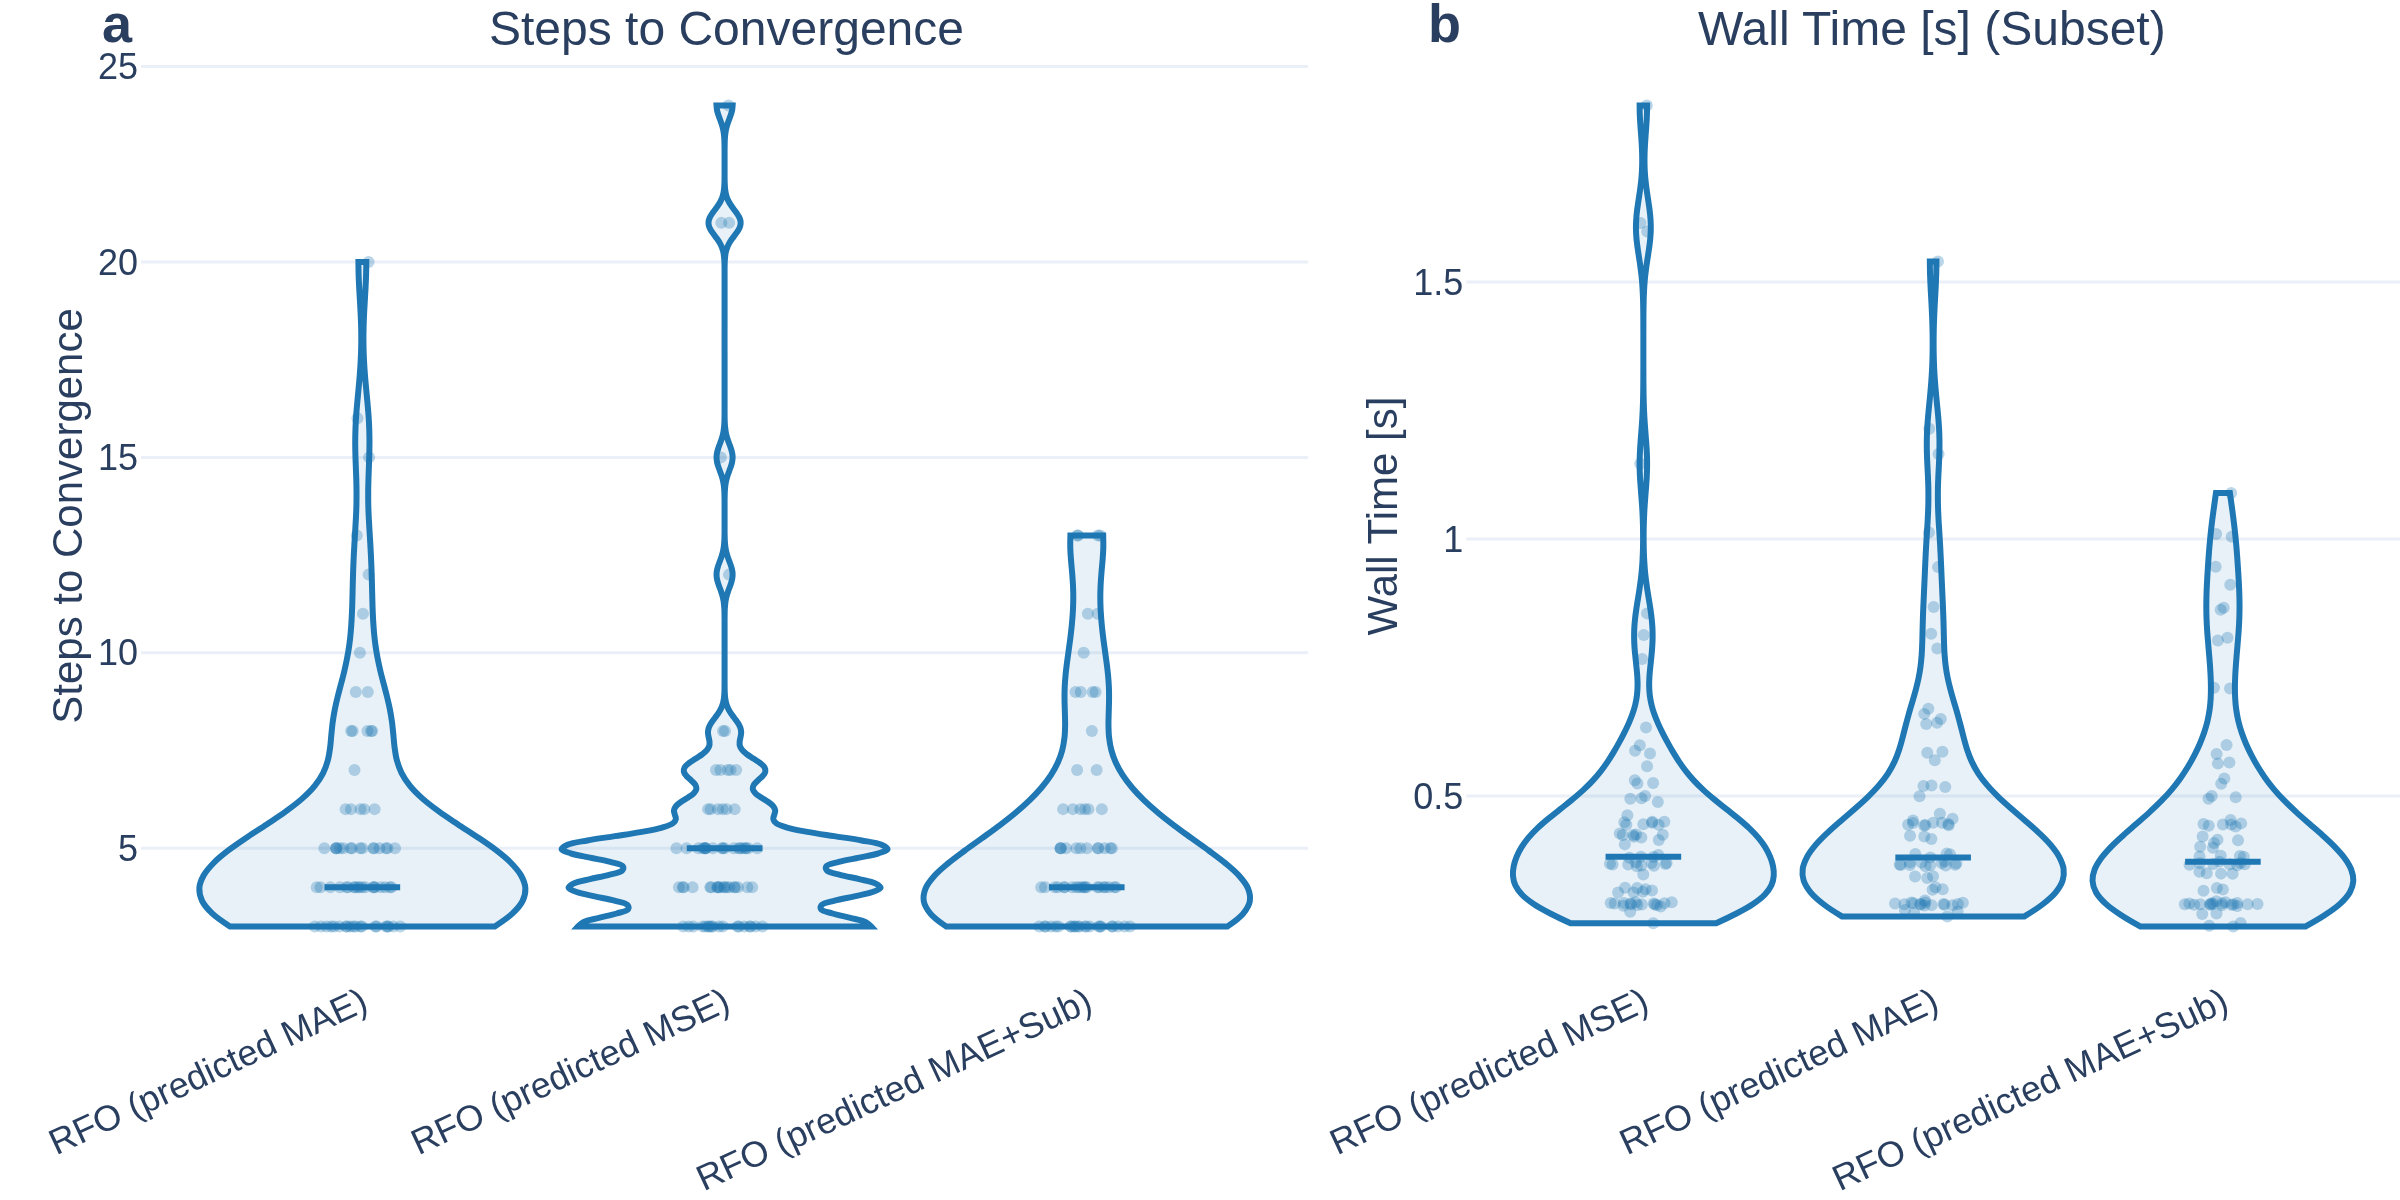
\includegraphics[width=0.75\linewidth]{plots/relaxations_lossablation.png}
    \caption{Geometry relaxation with HIP-EquiformerV2 trained using different loss functions}
    \label{fig:loss_relax}
\end{figure}

\begin{table}
\centering
\resizebox{0.7\textwidth}{!}{
\centering
\begin{tabular}{llll}
\toprule
Hessian & Model & ZPE MAE (Std) [eV] & $\Delta$ZPE MAE (Std) [eV] \\
\midrule
MSE & HIP-EquiformerV2 & 0.0008 (0.0012) & 0.0019 (0.0025) \\
MAE & HIP-EquiformerV2 & 0.0004 (0.0004) & \textbf{0.0013 (0.0019)} \\
MAE+Sub & HIP-EquiformerV2 & \textbf{0.0004 (0.0003)} & 0.0016 (0.0018) \\
\bottomrule
\end{tabular}
}
\caption{Zero-point energy by HIP-EquiformerV2 for different loss functions}
\label{tab:loss_zpe}
\end{table}

% TS search
\begin{table}
\centering
\resizebox{0.6\textwidth}{!}{
\centering
\begin{tabular}{llcccc}
\hline
Loss & Model & TS Success & RFO Converged & Both \\
\hline
MSE & HIP-EquiformerV2 & 718 & 669 & 659 \\
MAE & HIP-EquiformerV2 & 740 & 693 & 683 \\
MAE+Sub & HIP-EquiformerV2 & \textbf{750} & \textbf{705} & \textbf{698} \\
\hline
\end{tabular}
}
\caption{Transition state search with HIP-EquiformerV2 trained with different loss functions}
\label{tab:loss_tssearch}
\end{table}

\begin{table}
\centering
\resizebox{0.75\textwidth}{!}{
\centering
\begin{tabular}{lccccccc}
\hline
Name & TPR $\uparrow$ & FPR $\downarrow$ & FNR $\downarrow$ & TNR $\uparrow$ & Precision $\uparrow$ & Accuracy $\uparrow$&  Accuracy All $\uparrow$ \\
\hline
MSE  & 88\% & 11\%  & 12\%  & 89\% & 86\% & 89\% & 86\% \\
MAE  & 93\% & 7\%  & 7\%  & 93\% & 91\% & 93\% & 91\%  \\
MAE+Sub  & \textbf{93\%} & \textbf{6\%}  & \textbf{7\%}  & \textbf{94\%} & \textbf{92\%} & \textbf{94\%} & \textbf{92\%} \\
\hline
\end{tabular}
}
\caption{Identifying transition states (left) and any extrema (rightmost column) via frequency analysis using HIP-EquiformerV2 for different loss functions.}
\label{tab:loss_freqanalysis}
\end{table}



% \subsection{Computational cost compared to finite difference}
% \begin{figure}
%     \centering
%     \includegraphics[width=0.8\linewidth]{plots/speed_memory_finitedifference.png}
%     \caption{
%     \textbf{Computational cost.} Comparing (a) time and (b) memory of a forward without Hessians, with HIP, automatic differentiation (AD), finite difference Hessians. The memory for Forward Pass, FD Hessians, and HIP Hessians is nearly identical.
%     }
%     \label{fig:speedmemoryfinitedifference}
% \end{figure}
% \cite{wander2025accessing} showed that finite-difference Hessians obtained from finetuned MLIPs can increase success rates in transition state search for catalysis. The advantage of finite difference is that it does not require additional memory over a regular forward pass, and only force labels are needed for training. The limitation of finite-difference Hessians is their high computational cost. Like AD Hessians, finite difference requires $O(N^2)$ time, but with an even larger prefactor, as can be seen in Fig. \ref{fig:speedmemoryfinitedifference}.





\subsection{Training resources}
Training AD Hessians is exceptionally more expensive than training HIP.
The memory cost of computing loss gradients through the full  $3N\times3N$ Hessian is prohibitive. Instead, the baseline models from \cite{cui2025horm} randomly sample one or two columns of the Hessian via random Hessian-vector products at each training step. Despite this, training AD Hessians remains exceedingly expensive. The HORM paper states that they use 2 HVPs at a batch size of 128. Their checkpoint metadata shows a per-device batch size of 8, suggesting a 16$\times$ A30 GPU setup for 1 million gradient steps.
In contrast, we trained HIP on a single H100 GPU for 500k steps. Additionally, each HIP training step costs 1/5 as much as AD Equiformer training on our hardware. Finally, we observe that HIP fully converges after 300-500k training steps, whereas AD Hessians require multiple steps due to the limited supervision and the inability to use the full Hessian.

\begin{table}[h]
\centering
\renewcommand{\arraystretch}{1.6} % Adjust row height
\resizebox{0.8\textwidth}{!}{ % Resize to fit the page width
\begin{tabular}{lccccccc}
\hline
\textbf{Model} & Hessian Columns & Batch Size &
BZ / GPU & GPU & \# GPUs & Training Steps \\
\hline
AlphaNet            & 1 & 32  & 16 & H20 & 2  & 688,000 \\
LeftNet-CF          & 1 & 64  & 16 & A30 & 8  & 192,000 \\
LeftNet-DF          & 2 & 64  & 16 & A30 & 8  & 120,000 \\
EquiformerV2 (E-F)  & 0 & 128 & 8  & A30 & 16 & 384,000 \\
EquiformerV2        & 2 & 128 & 8  & A30 & 16 & 1,008,000 \\
\hline
HIP-EquiformerV2        & 3N (all) & 128 & 128 & H100 & 1 & 500,000 \\
\hline
\end{tabular}
}
\caption{\textbf{Summary of training resources.} Comparing HIP to checkpoints from HORM \citep{cui2025horm}.}
\label{tab:traingpu}
\end{table}

\subsection{ZPE definition}
\[
\Delta \mathrm{ZPE}_{m}
= \mathrm{ZPE}_{m}(\text{product}) - \mathrm{ZPE}_{m}(\text{reactant}).
\]
The $\Delta\Delta$DFT error for a model is
$$
\Delta\Delta \mathrm{ZPE}
= \bigl|\Delta \mathrm{ZPE}_{\text{model}} - \Delta \mathrm{ZPE}_{\text{DFT}}\bigr|.
$$
The computational protocol is provided in the main Methods.

\subsection{Glycine proton-transfer surface}
The computational protocol is provided in the main Methods.

\begin{figure}
    \centering
    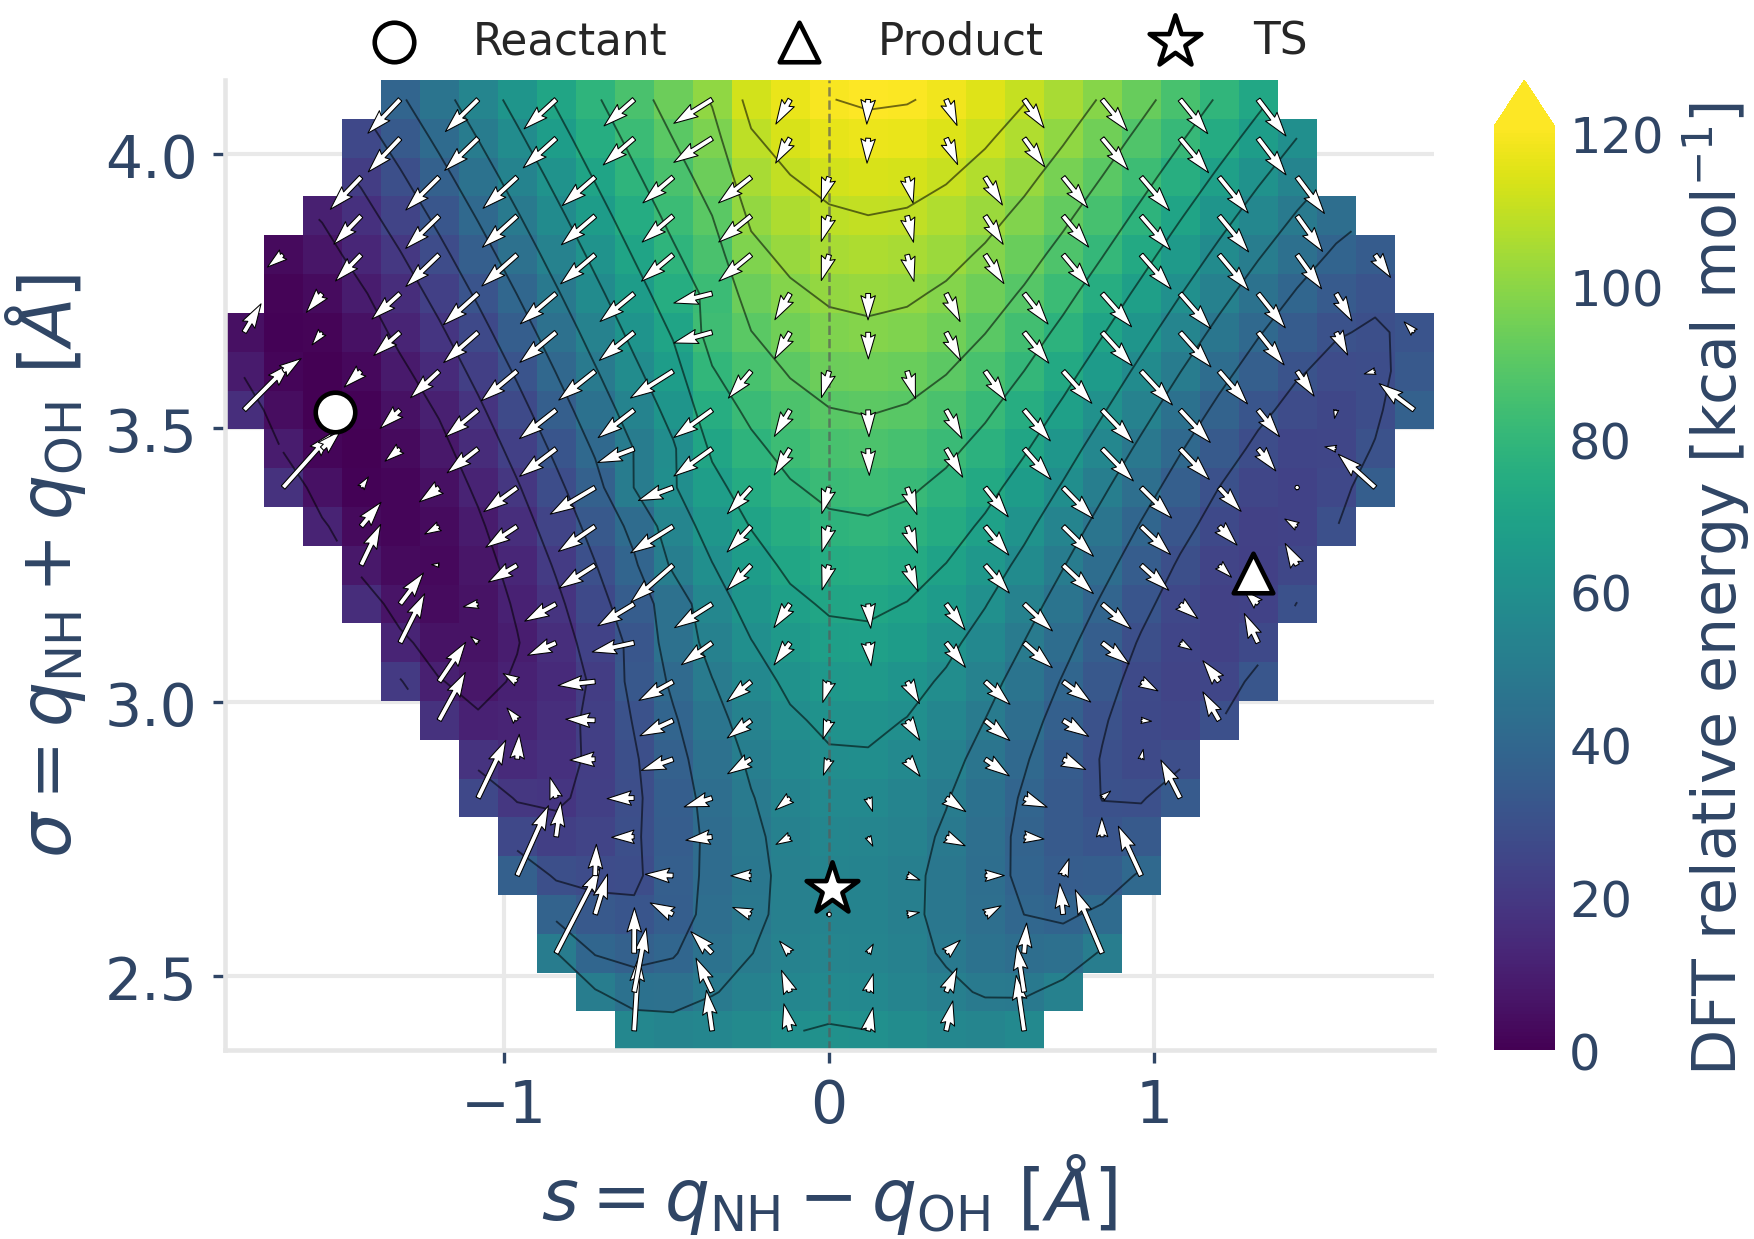
\includegraphics[width=0.52\linewidth]{plots/glycine_dftrelaxed_forcefield.png}
    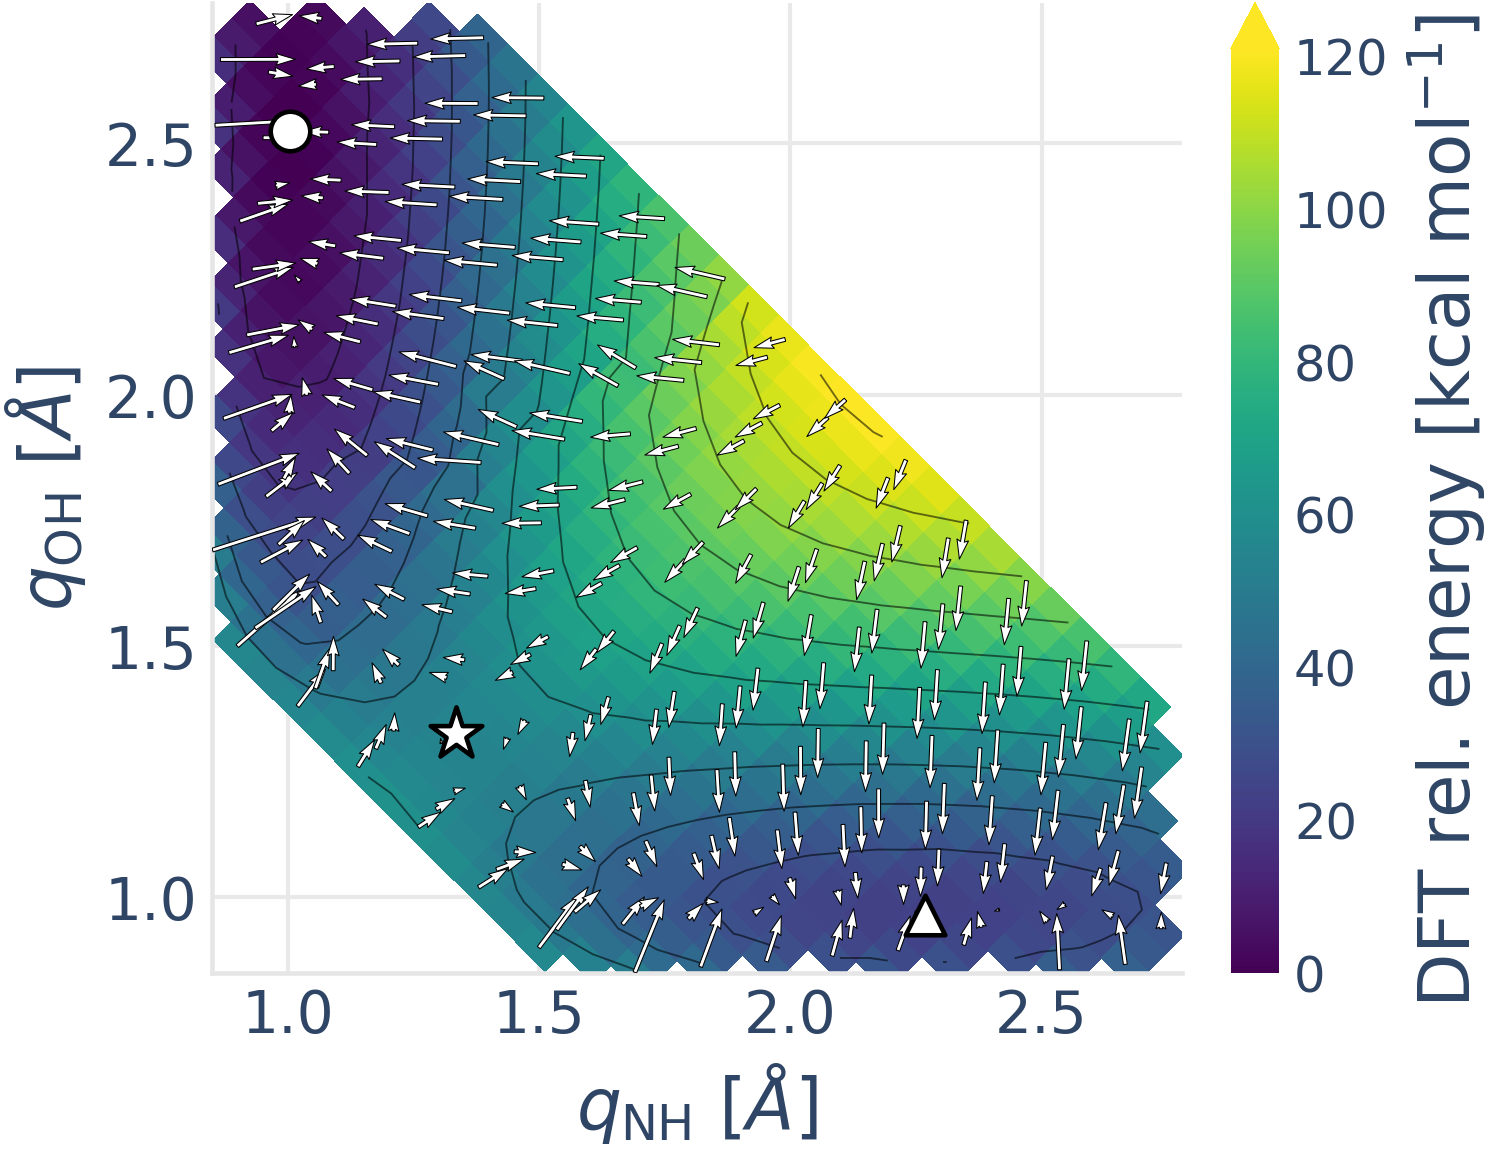
\includegraphics[width=0.45\linewidth]{plots/glycine_dftrelaxed_forcefield_q.png}
     \caption{
     \textbf{Glycine.} 
     2D collective variable energy surface at $\omega$B97X/6-31G(d), with forces shown as arrows. 
     % The star marks the transition state. The top right corner corresponds to the hydrogen dissociating from the molecule.
     The DFT-optimized reactant and product contain no imaginary frequencies, while the DFT transition-state optimization yields one imaginary frequency, confirming the expected minimum/first-order-saddle classifications.
     }
     \label{fig:glycine_forcefield}
\end{figure}

\bibliography{sn-bibliography}

\end{document}
